\apendice{Estudio experimental}



\section{Cuaderno de trabajo.}

\subsection{Comité de Ética}
El proyecto comenzó con la obtención de la aprobación ética necesaria para el uso de imágenes clínicas. Se solicitó la autorización del CEIM del HUBU para acceder a imágenes de ecografía obstétrica. 

Para ello, se redactó inicialmente un documento que describía los objetivos del estudio, la metodología y el tratamiento de los datos. Durante el proceso de evaluación, el CEIM solicitó aclaraciones y modificaciones, las cuales fueron incorporadas y respondidas puntualmente. Además, se añadieron documentos complementarios como la hoja de información al paciente y el consentimiento informado, garantizando el cumplimiento ético del estudio.

La aprobación fue concedida el 6 de mayo de 2025, con el número de registro de CEIM 3246, en el marco del proyecto titulado "Detección de estructuras craneales en ecografías en distintas etapas del embarazo". Todas las pacientes firmaron el consentimiento informado, y las imágenes utilizadas provinieron de ecografías realizadas en el seguimiento gestacional habitual, sin pruebas adicionales con fines exclusivamente investigativos.

\subsection{Primeras pruebas y modelos}

En las etapas iniciales del proyecto se exploraron diversas técnicas y modelos de segmentación de imágenes médicas con el objetivo de identificar la estrategia más adecuada para el problema clínico planteado.
\begin{itemize}
    \item \textbf{YOLOv8}: Se evaluó la viabilidad de utilizar YOLOv8 \footnote{\url{https://docs.ultralytics.com/es/tasks/segment/}}, en su variante de segmentación, un modelo desarrollado por Ultralytics que permite la segmentación en tiempo real de imágenes médicas. Sin embargo, el ruido característico de estas imágenes y la gran variabilidad entre ellas afectó negativamente a su rendimiento.
    \item \textbf{DeepLabV3+}: También se probaron modelos basados en la arquitectura DeepLabV3+, reconocida por su eficacia. No obstante, sus resultados no fueron suficientemente precisos para tareas de segmentación detallada.
    \item \textbf{Segment Anything Model (SAM)}: Se utilizó SAM para integrar una segmentación inicial del contorno cerebral, con el objetivo posterior de aplicar una segmentación más fina sobre las estructuras internas. Sin embargo, los resultados tampoco fueron satisfactorios debido a la naturaleza borrosa y variable de las ecografías fetales.
\end{itemize}
Por último, se optó por utilizar la librería \texttt{segmentation\_models\_pytorch}, que ofrece la implementación de un mismo modelo para el uso de varias arquitecturas como \texttt{Unet}, \texttt{Unet++}, \texttt{Linknet}, \texttt{FPN}, \texttt{MAnet}, \texttt{PSPNet} basados en redes convolucionales profundas. Esta elección permitió obtener una mayor precisión.

\subsection{Desarrollo de la aplicación local.}
Una vez entrenado el modelo y almacenado el mejor resultado mediante la funcionalidad de \texttt{checkpoints}, utilizando el conjunto de datos clínicos obtenido del HUBU, se procedió al desarrollo de una aplicación local con el objetivo de facilitar su uso por parte del personal clínico.

La aplicación fue desarrollada con \textit{Streamlit}, una biblioteca de Python que permite la creación de interfaces gráficas de manera sencilla. La versión inicial permitía cargar imágenes de ecografía y visualizar las predicciones de segmentación generadas por el modelo.

Posteriormente, tras recibir sugerencias del profesional médico colaborador, se incorporaron funcionalidades adicionales, como la visualización de la máscara \textit{ground truth} (cuando estaba disponible) y la generación automática de informes en formato PDF con los resultados obtenidos.

Esta aplicación local permitió ajustar la interfaz en función del uso clínico, situando cada elemento en la disposición más adecuada para una experiencia intuitiva y centrada en el usuario.

\subsection{Proceso de despliegue a la nube.}
Para el acceso remoto a la herramienta, el modelo fue desplegado en la nube. Para ello, tanto los datos como el modelo y el código fueron subidos al repositorio de GitHub del proyecto \href{https://github.com/eirarodriguez/fetal_brain_segmentation} {fetal\_brain\_segmentation}. 

Posteriormente, utilizando la plataforma \textit{Streamlit Community Cloud}, que permite la ejecución directa del código desde un repositorio, se generó una URL pública que permite el acceso a la aplicación sin necesidad de instalación local, facilitando así su evaluación y uso desde cualquier ubicación.


\subsection{Validación del personal clínico.} 
Se contó con la colaboración de un profesional médico de la unidad de obstetricia, quien participó activamente en la validación de cada una de las etapas del proyecto.

Para validar el modelo de segmentación, se le enviaron los informes generados automáticamente con los resultados obtenidos por cada arquitectura evaluada. 

Además, se le consultó sobre la relevancia clínica para segmentar el cuarto ventrículo, estructura que inicialmente formaba parte del conjunto de clases, para cuya detección resultó poco consistente debido a su pequeño tamaño. Tras su evaluación, se concluyó que no era esencial para el propósito clínico del proyecto, por lo que se decidió centrar la segmentación en estructuras de mayor importancia.

Una vez desarrollada la aplicación, se enviaron al profesional videos explicativos sobre su funcionamiento. Finalmente, tras incorporar todas las funcionalidades propuestas, se compartió la URL de la versión desplegada, la cual fue revisada y se considera satisfactoria para su uso.

\section{Configuración y parametrización de las técnicas.}

Durante el desarrollo del modelo de segmentación, se ajustaron progresivamente los parámetros y la configuración del entrenamiento con el objetivo de mejorar la precisión sin comprometer la eficiencia computacional ni el cumplimiento clínico del proyecto.

\subsection{Arquitectura y encoder} 

La arquitectura seleccionada fue \texttt{U-Net}, junto con el encoder \texttt{ResNeXt50\_32x4d}, preentrenado en ImageNet. Esta combinación demostró un rendimiento sólido en las pruebas realizadas en el conjunto clínico disponible.

\subsection{Función de pérdida}
Para la optimización del modelo se utilizó la función de pérdida \texttt{DiceLoss} en modo \texttt{multiclass}. Esta función está basada en el coeficiente Dice, una métrica que cuantifica la similitud entre dos conjuntos, en este caso, la máscara predicha y la máscara de referencia.

También fue configurada para trabajar directamente con los \textit{logits} del modelo, permitiendo una optimización directa y estable desde el inicio del entrenamiento.

\subsection{Parámetros de entrenamiento}
Los parámetros de entrenamiento se definieron a partir de configuraciones base ampliamente utilizadas en segmentación multiclase con redes convolucionales profundas, partiendo del código de la comunidad oficial de \texttt{segmentation\_models\_pytorch}. Posteriormente, fueron ajustados para adaptarse a las particularidades de las imágenes clínicas en este proyecto.
\begin{itemize}
    \item \textbf{Épocas (\texttt{max\_epochs})}: se estableció un límite de 200 épocas como máximo. Este valor alto permite al modelo un entrenamiento profundo, pero se controló mediante \texttt{EarlyStopping} para evitar el sobreajuste, deteniendo el proceso automáticamente si la pérdida no mejoraba en 30 épocas consecutivas. 
    \item \textbf{Tamaño del batch (\texttt{Batch size})}: se utilizó un batch size de 1, lo cual es común en tareas de segmentación médica, especialmente cuando se trabaja con imágenes grandes o cuando se dispone de recursos computacionales limitados. Esta configuración permite mantener la carga de memoria dentro de los límites de la GPU utilizada.
    \item \textbf{Optimizador (Adam)}: Se seleccionó el optimizador \texttt{Adam}, ampliamente adoptado en redes neuronales profundas. Su principal ventaja es que adapta la tasa de aprendizaje de forma individual para cada parámetro, lo que la hace especialmente útil en escenarios con ruido o desbalances entre clases, como lo son las ecografías médicas.
    \item \textbf{Tasa de aprendizaje (\texttt{learning rate})}: Se fijó un valor inicial de 0,0002. Este valor moderadamente bajo favorece una convergencia estable, especialmente en los primeros pasos del entrenamiento. 
    \item \textbf{Scheduler}: Se aplicó un scheduler de tipo coseno, que reduce progresivamente la tasa de aprendizaje hasta un mínimo de 0,00001. Esta estrategia ayuda a refinar los pesos del modelo en fases avanzadas del entrenamiento, evitando que quede atrapado en mínimos poco óptimos.
\end{itemize}
\subsection{Callbacks de entrenamiento}
\begin{itemize}
    \item \textbf{EarlyStopping}: Se utilizó con una paciencia de 30 épocas, monitorizando la pérdida de validación. Esta estrategia permitió evitar sobreajuste y reducir el tiempo de entrenamiento.
     \item \textbf{ModelCheckpoint}: Se guardó automáticamente el modelo con la menor pérdida de validación registrada durante el entrenamiento, facilitando su posterior evaluación y despliegue.
\end{itemize}
\subsection{Augmentaciones y reprocesamiento}
Para mejorar la capacidad de generalización del modelo, se aplicaron técnicas de \textit{data aumentation} durante el entrenamiento, incluyendo rotaciones, desplazamientos, ajustes de brillo y contraste, así como normalización. Durante la validación y prueba, se utilizó únicamente la normalización estándar.

\section{Detalle de resultados.}
En la carpeta de Resultados, disponible en el repositorio de GitHub del proyecto, se incluyeron los informes generados sobre el conjunto de prueba. Cada informe contiene:
\begin{itemize}
    \item Cuatro imágenes de prueba, con su ground truth y la segmentación predicha por el modelo.
    \item Una tabla con métricas por clase (precisión e IoU).
    \item El promedio de estas métricas para cada imagen.
    \item La evolución de la función de pérdida durante el entrenamiento.
\end{itemize}

Estos elementos permitieron realizar una evaluación tanto cuantitativa como cualitativa del comportamiento de cada modelo.

En la Tabla \ref{tab:resultados_earlystopping}, se presenta una comparativa de métricas medias para arquitectura. Los resultados se obtuvieron aplicando técnicas de \textit{data augmentation} y \textit{early stopping} durante el entrenamiento, y fueron evaluados sobre el conjunto de prueba. 

\begin{table}[h]
    \centering
    \begin{tabular}{lcc}
    \textbf{Arquitectura} & \textbf{Precisión media (\%)} & \textbf{IoU media (\%)} \\
    \hline
    U-Net             & 70,74 & 63,69\\
    U-Net++           & 67,07 & 62,46\\
    FPN               & 70,77 & 60,23\\
    PSPNet            & 15,06 & 12,11\\
    LinkNet           & 71,12 & 60,32\\
    MAnet             & 61,49 & 55,62\\
    \hfill
    \end{tabular}
    \caption{Comparativa de métricas medias por arquitectura sobre el conjunto de prueba con \textit{early stopping}.} \label{tab:resultados_earlystopping}
\end{table}

El modelo U-Net alcanzó una IoU media del 63,69\%, lo que confirma su capacidad para segmentar con precisión estructuras cerebrales en ecografías obstétricas, superando consistentemente a otras arquitecturas evaluadas. Este valor se considera adecuado dentro del contexto clínico del proyecto, donde una IoU superior al 60\% permite una interpretación fiable por parte del personal médico.

Entre todos los modelos evaluados, U-Net obtuvo el mejor rendimiento en términos de IoU media, lo que respalda su elección como arquitectura base en tareas de segmentación médica. Sin embargo, U-Net++ y LinkNet también presentaron resultados competitivos, ligeramente por debajo.

Por el contrario, PSPNet mostró un rendimiento significativamente inferior, lo que evidencia su inadecuación para este tipo de imágenes, posiblemente debido a su diseño más orientado a escenas urbanas complejas y no a estructuras anatómicas.

A partir de esta comparativa, se seleccionaron tres arquitecturas representativas para un análisis más detallado:

\begin{itemize}
    \item \textbf{U-Net}: como referencia estándar, por ser la arquitectura con mayor IoU media y comportamiento robusto.
    \item \textbf{LinkNet}: por su precisión competitiva y eficiencia computacional.
    \item \textbf{PSPNet}: como ejemplo de arquitectura menos adecuada, dada su baja precisión y capacidad de segmentación en este dominio.
\end{itemize}

En las Figuras \ref{fig:comparacion_unet}, \ref{fig:comparacion_linknet} y \ref{fig:comparacion_pspnet}, se muestran visualizaciones de las predicciones generadas por estas tres arquitecturas, comparando la imagen original, la máscara real y la predicción del modelo.

\begin{figure}[h]
    \centering
    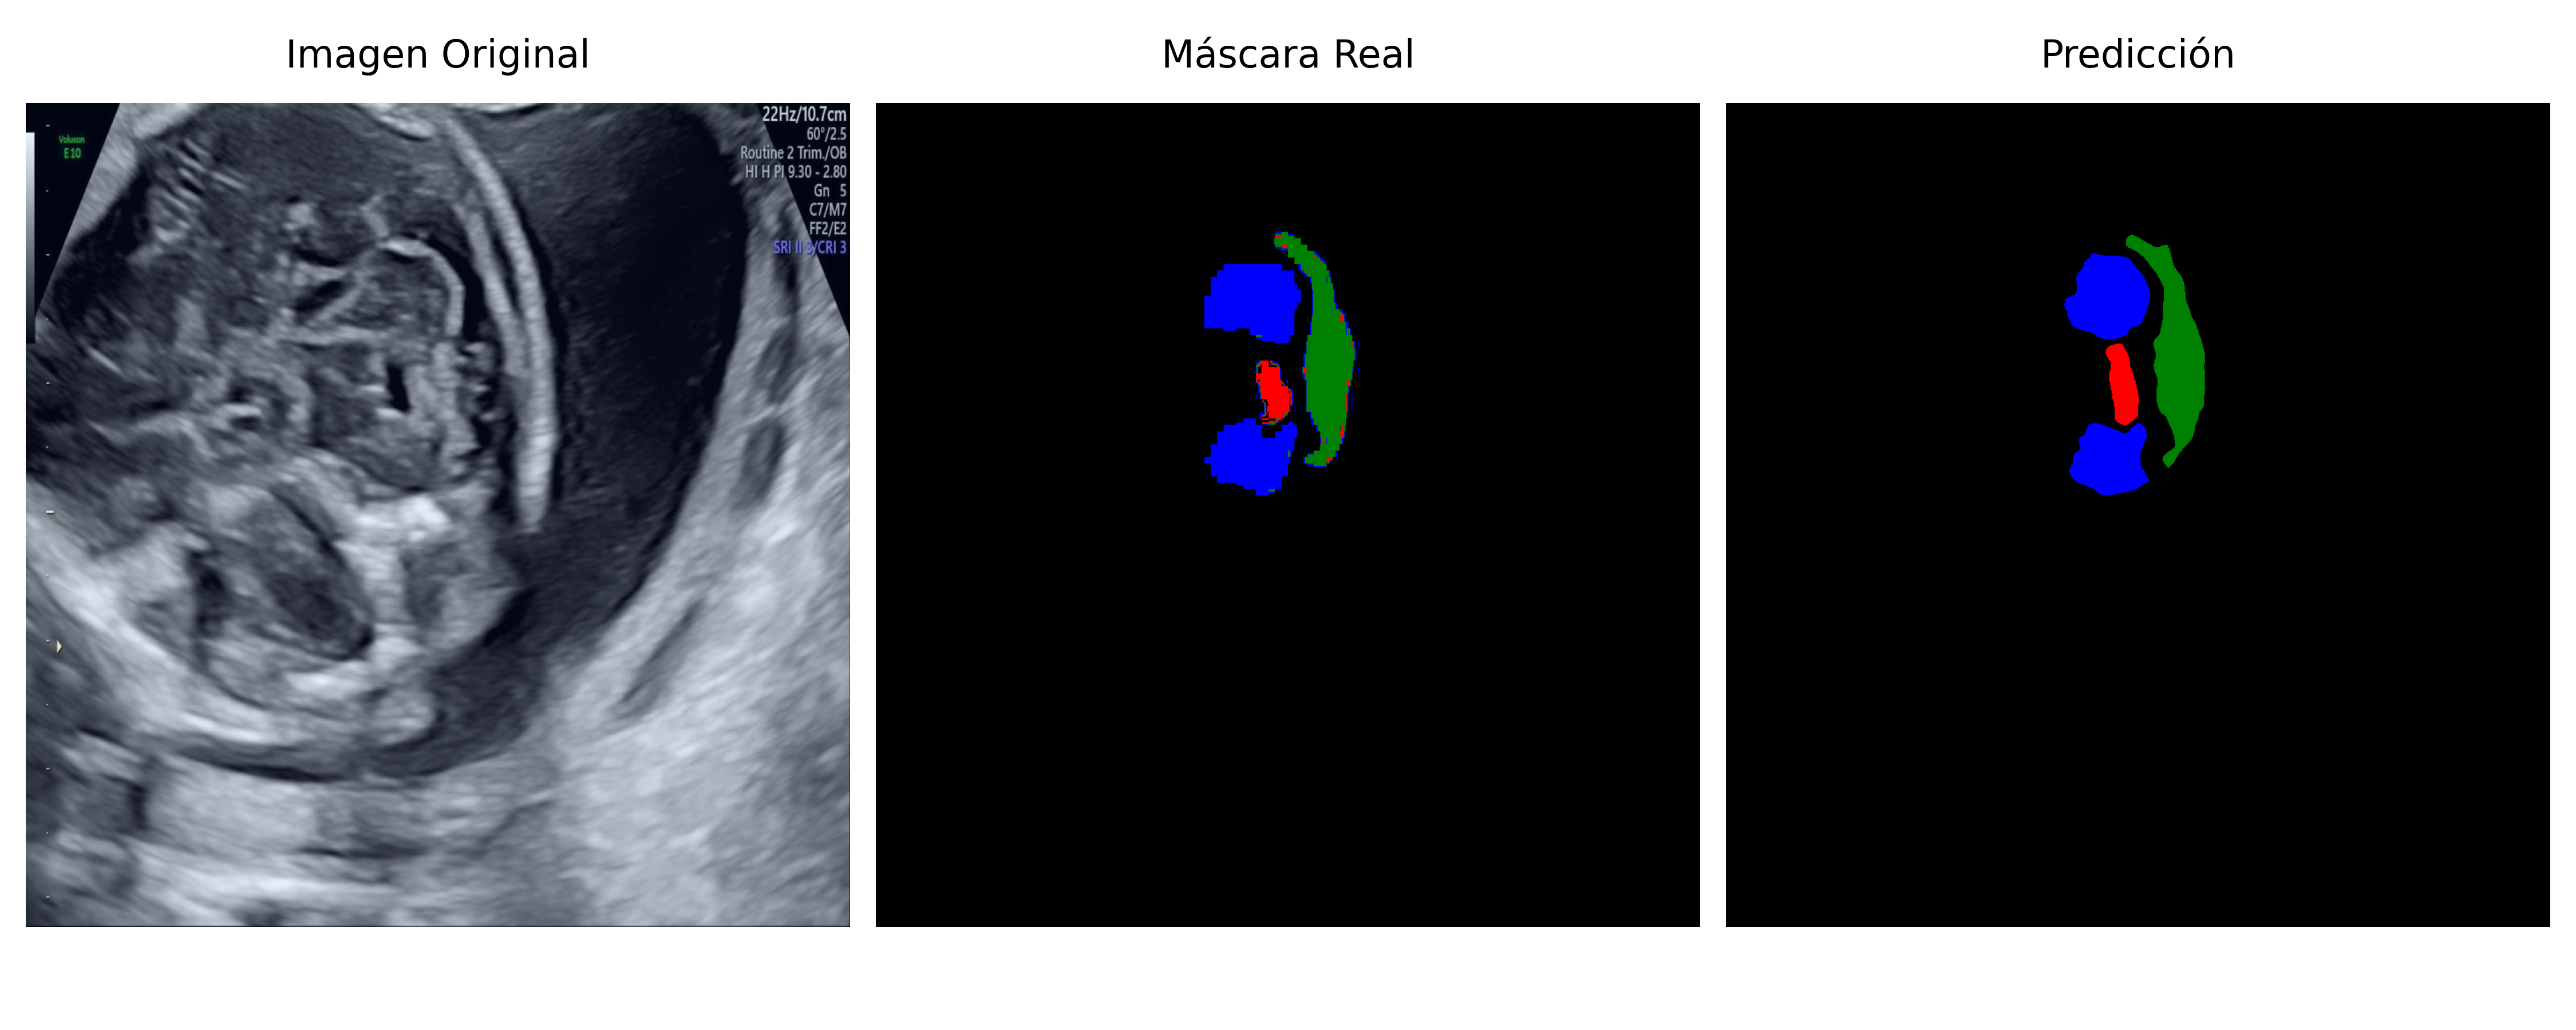
\includegraphics[width=1\textwidth]{img/image1_unet.png}
    \caption{Comparación visual de la segmentación generada por U-Net. De izquierda a derecha: imagen original, ground truth, predicción del modelo. }
    \label{fig:comparacion_unet}
\end{figure}

\begin{figure}[h]
    \centering
    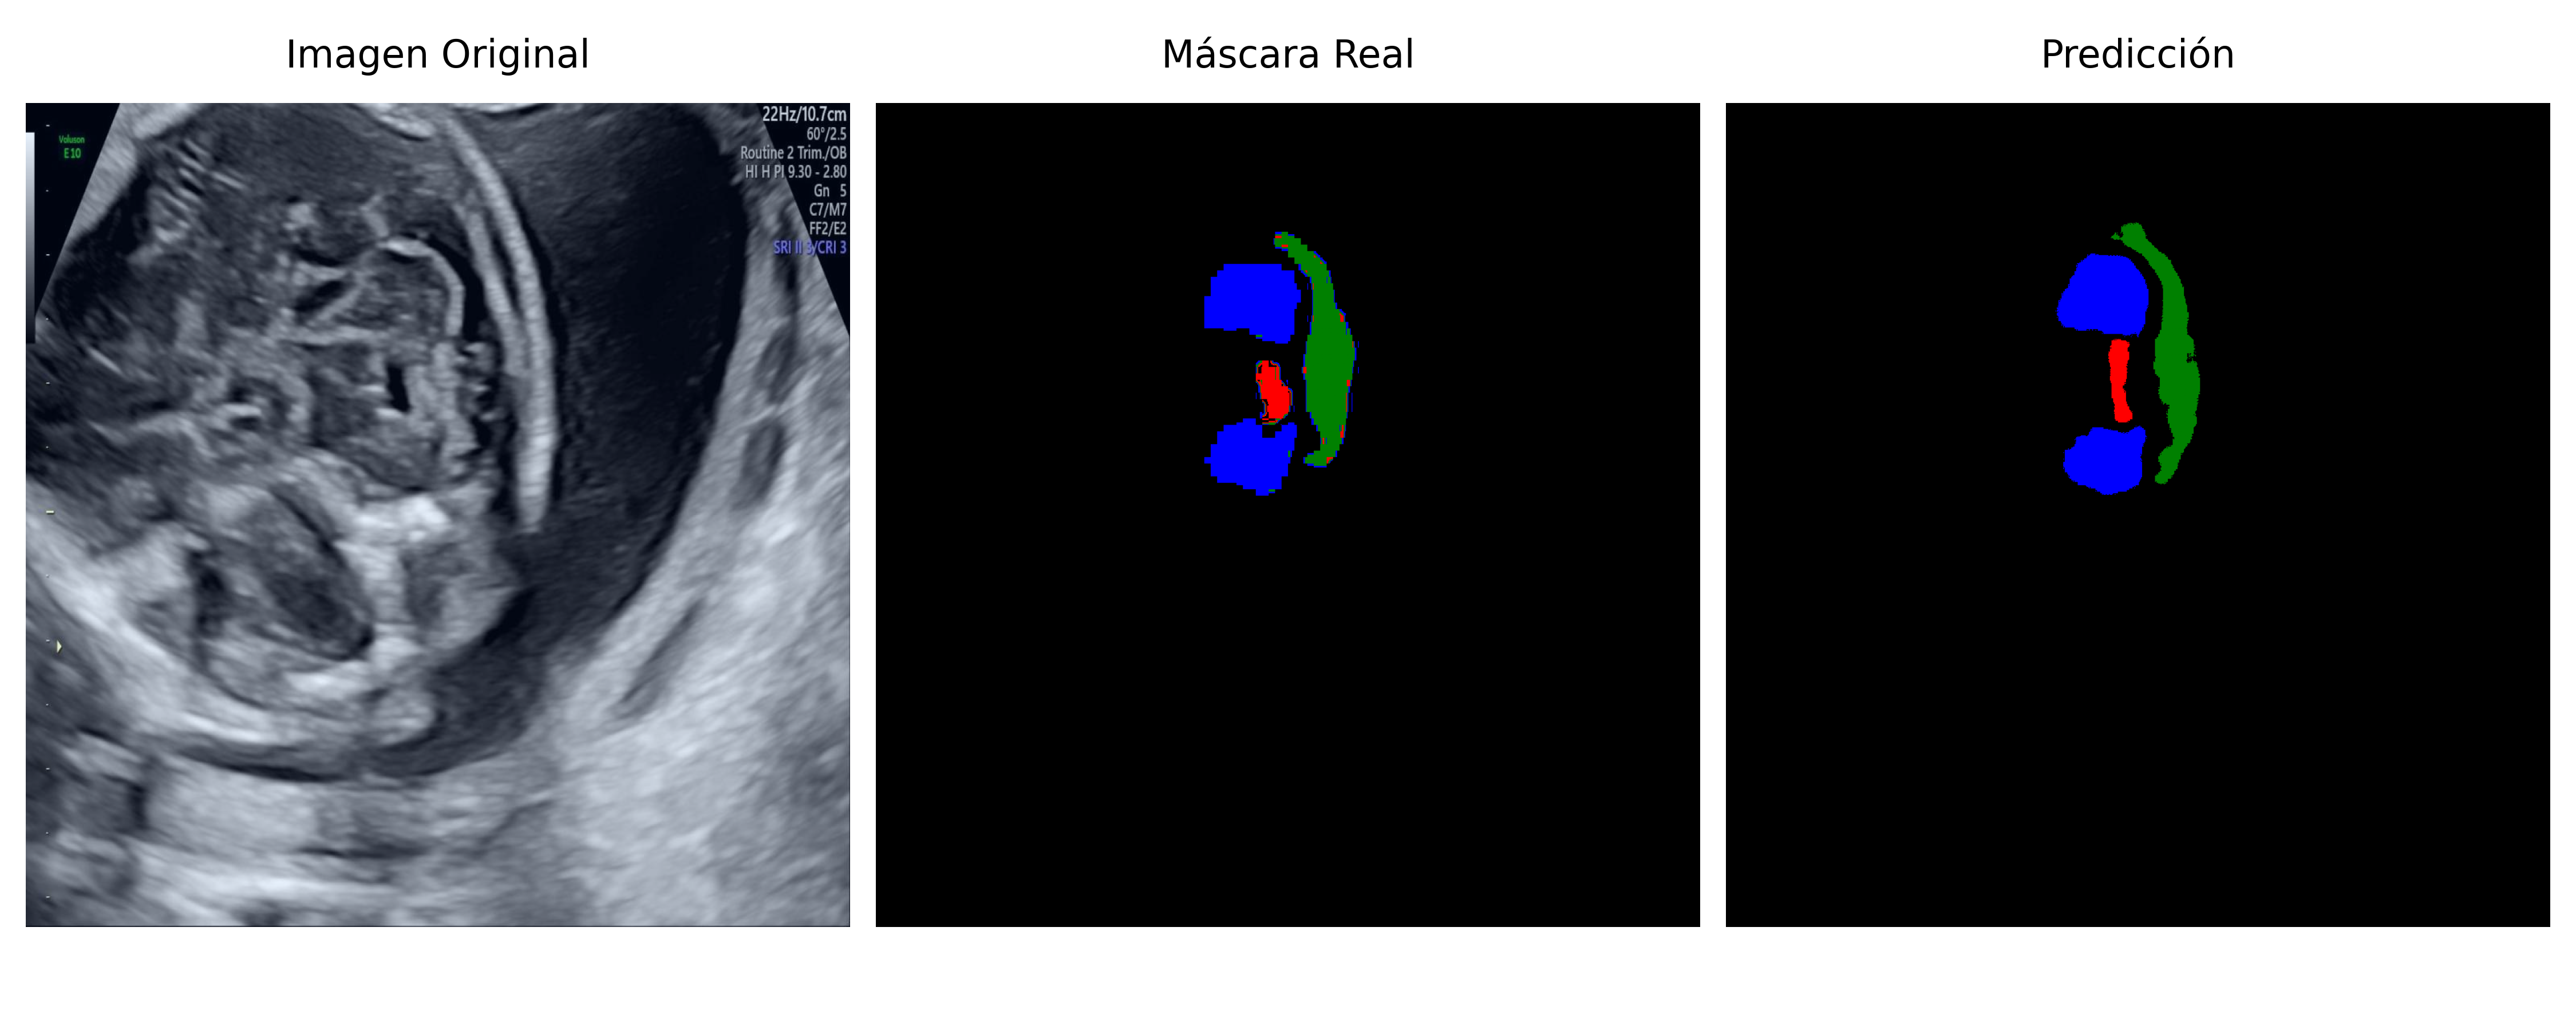
\includegraphics[width=1\textwidth]{img/image1_linknet.png}
    \caption{Comparación visual de la segmentación generada por LinkNet. De izquierda a derecha: imagen original, ground truth, predicción del modelo.}
    \label{fig:comparacion_linknet}
\end{figure}

\begin{figure}[h]
    \centering
    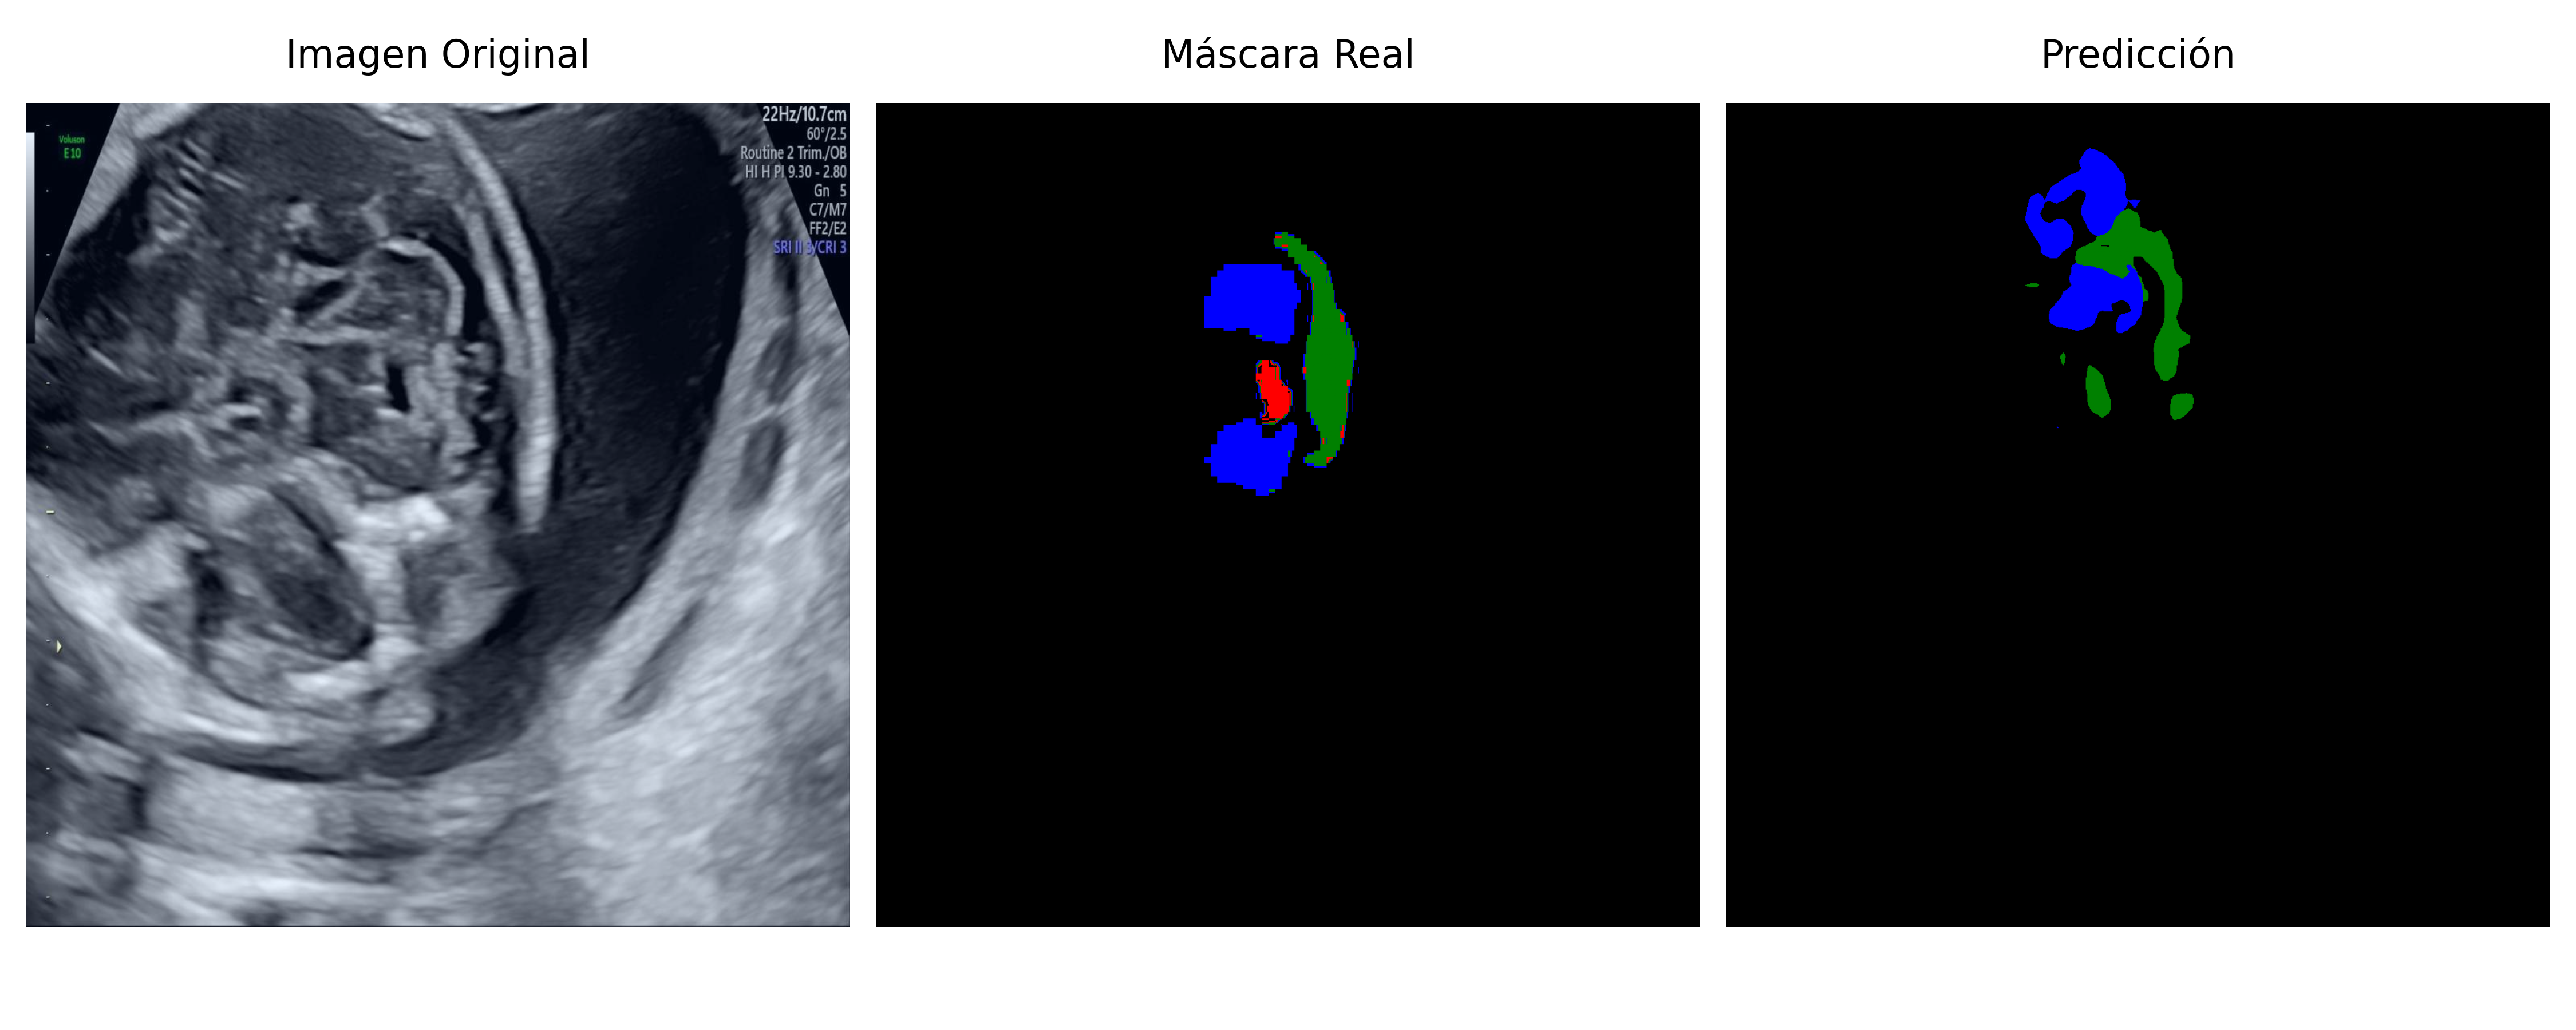
\includegraphics[width=1\textwidth]{img/image1_pspnet.png}
    \caption{Comparación visual de la segmentación generada por PSPNet. De izquierda a derecha: imagen original, ground truth, predicción del modelo.}
    \label{fig:comparacion_pspnet}
\end{figure}

Estas comparaciones permiten identificar las diferencias en el comportamiento de cada red. Mientras que U-Net consigue representar con bastante fiabilidad las estructuras del cerebelo, PSPNet falla al captar los entornos y tiende a subsegmentar o ignorar regiones relevantes.

Con base en este análisis, se optó por utilizar U-Net como modelo principal para la interfaz final, debido a su mayor IoU media y a la calidad de sus predicciones visuales.

Las visualizaciones adicionales incluidas en las Figuras \ref{fig:comparacion_unet2}, \ref{fig:comparacion_unet3} y \ref{fig:comparacion_unet4} respaldan el buen desempeño de U-Net, mostrando una segmentación consistente y adaptada a las variaciones presentes en las imágenes ecográficas.

\begin{figure}[h]
    \centering
    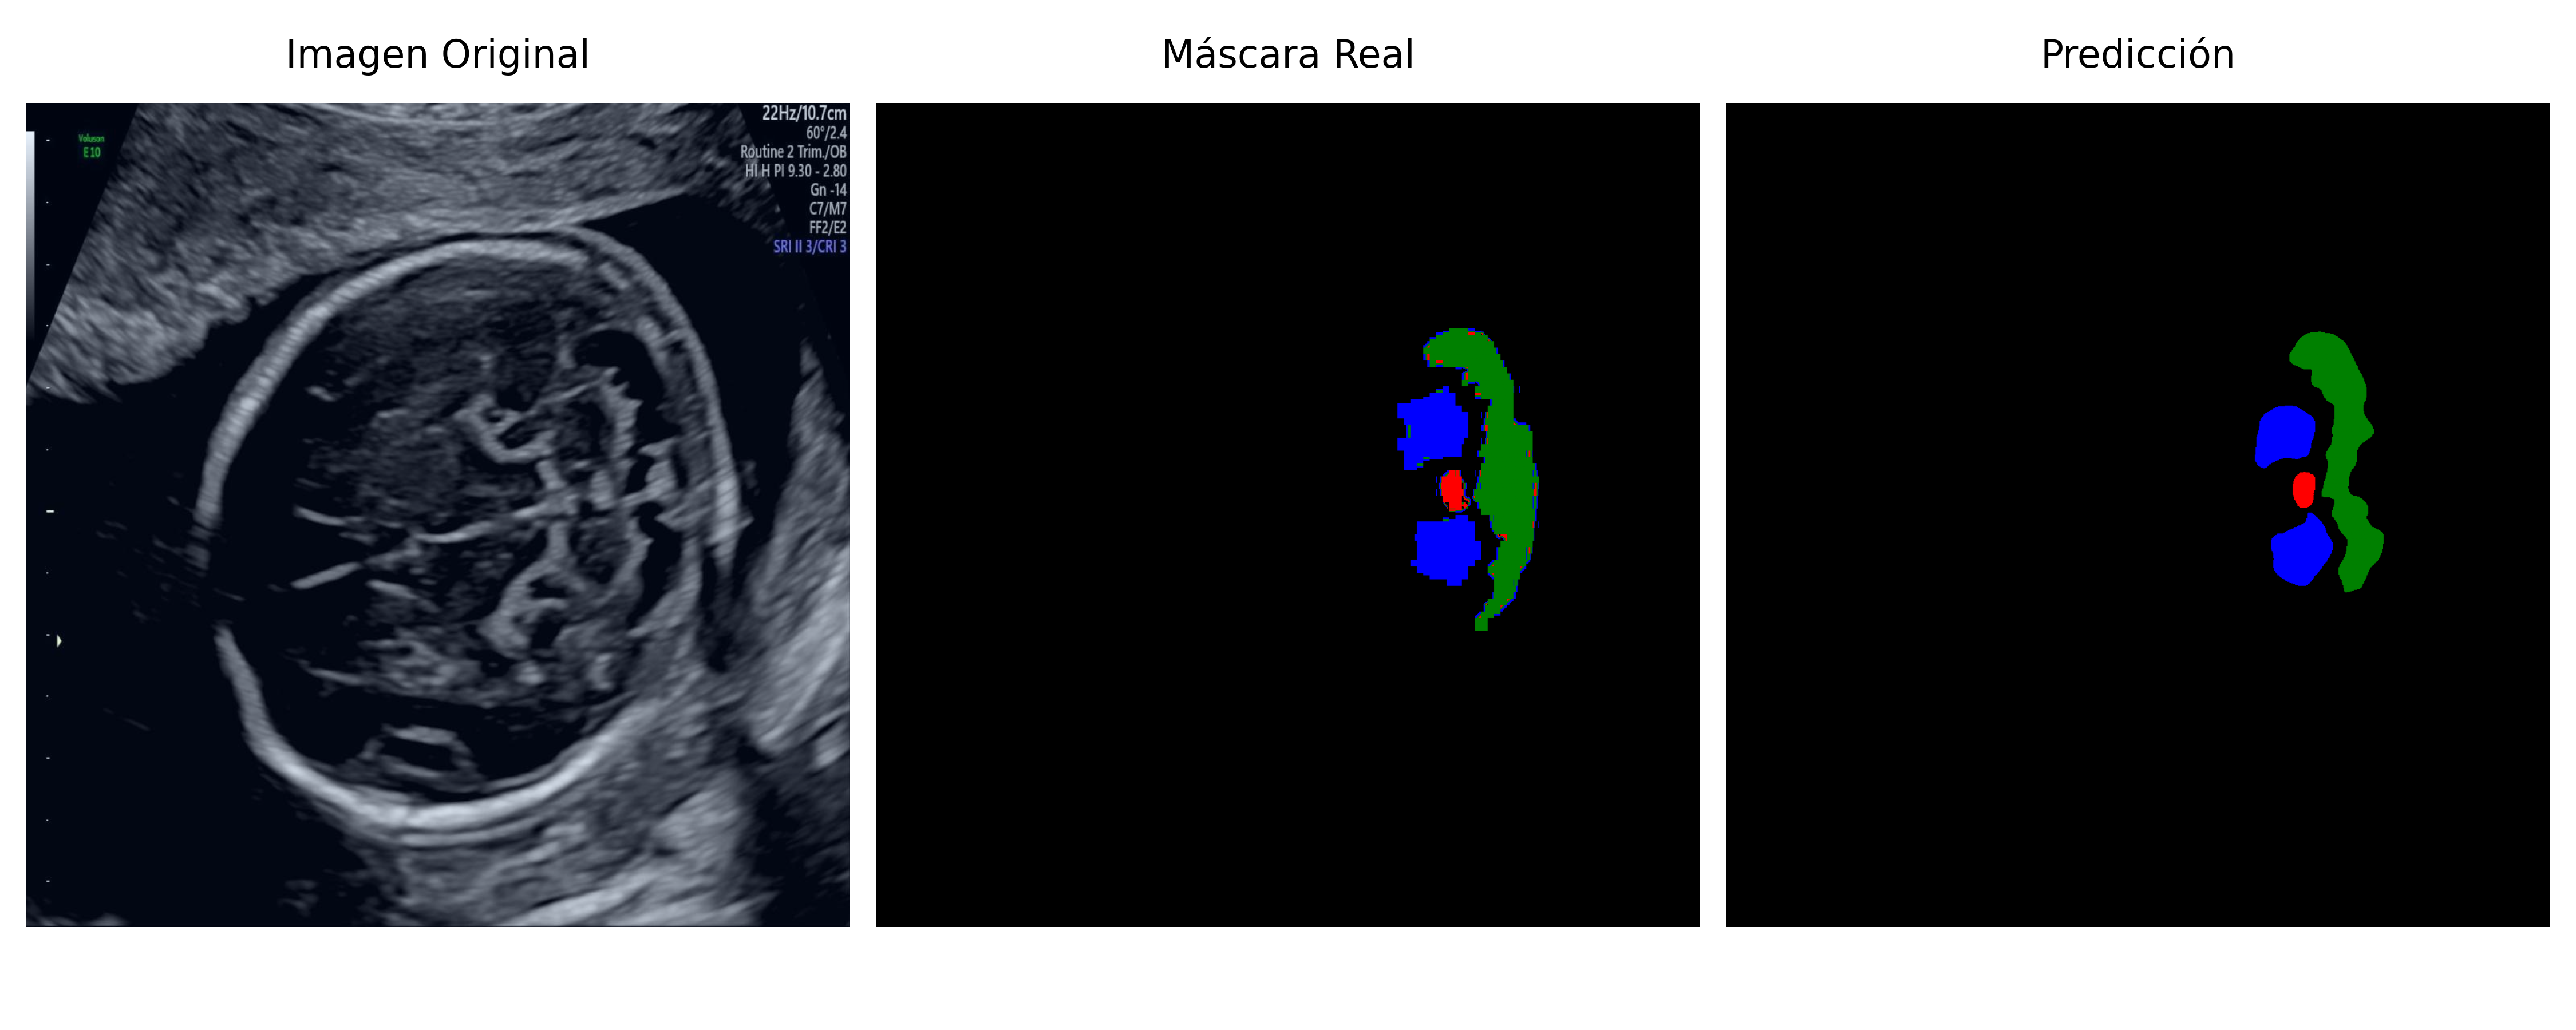
\includegraphics[width=1\textwidth]{img/image2_unet.png}
    \caption{Ejemplo adicional de segmentación con U-Net.}
    \label{fig:comparacion_unet2}
\end{figure}

\begin{figure}[h]
    \centering
    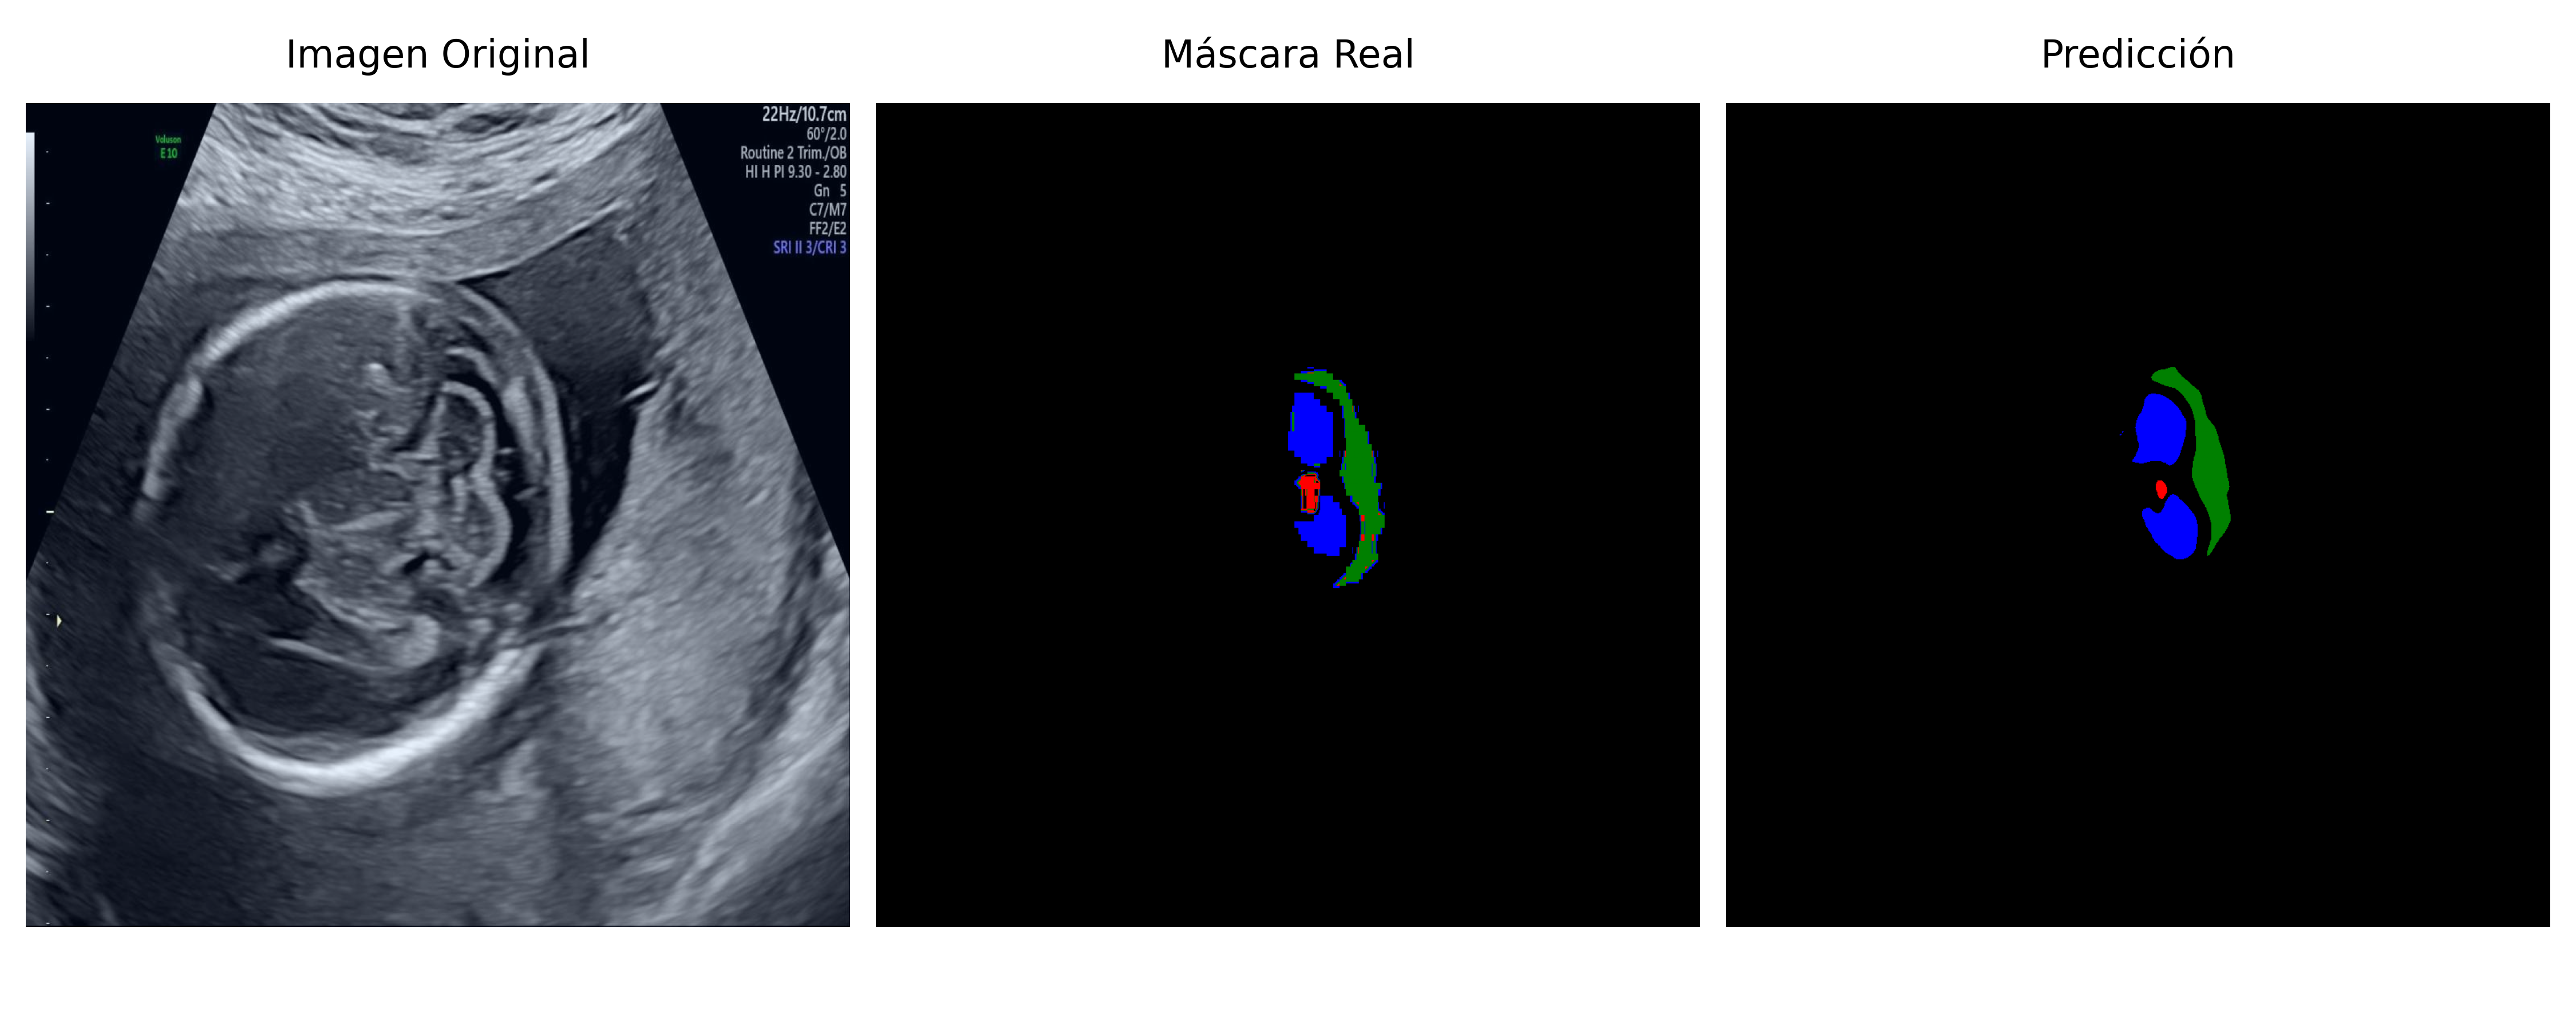
\includegraphics[width=1\textwidth]{img/image3_unet.png}
    \caption{Segunda visualización de resultados con U-Net.}
    \label{fig:comparacion_unet3}
\end{figure}

\begin{figure}[h]
    \centering
    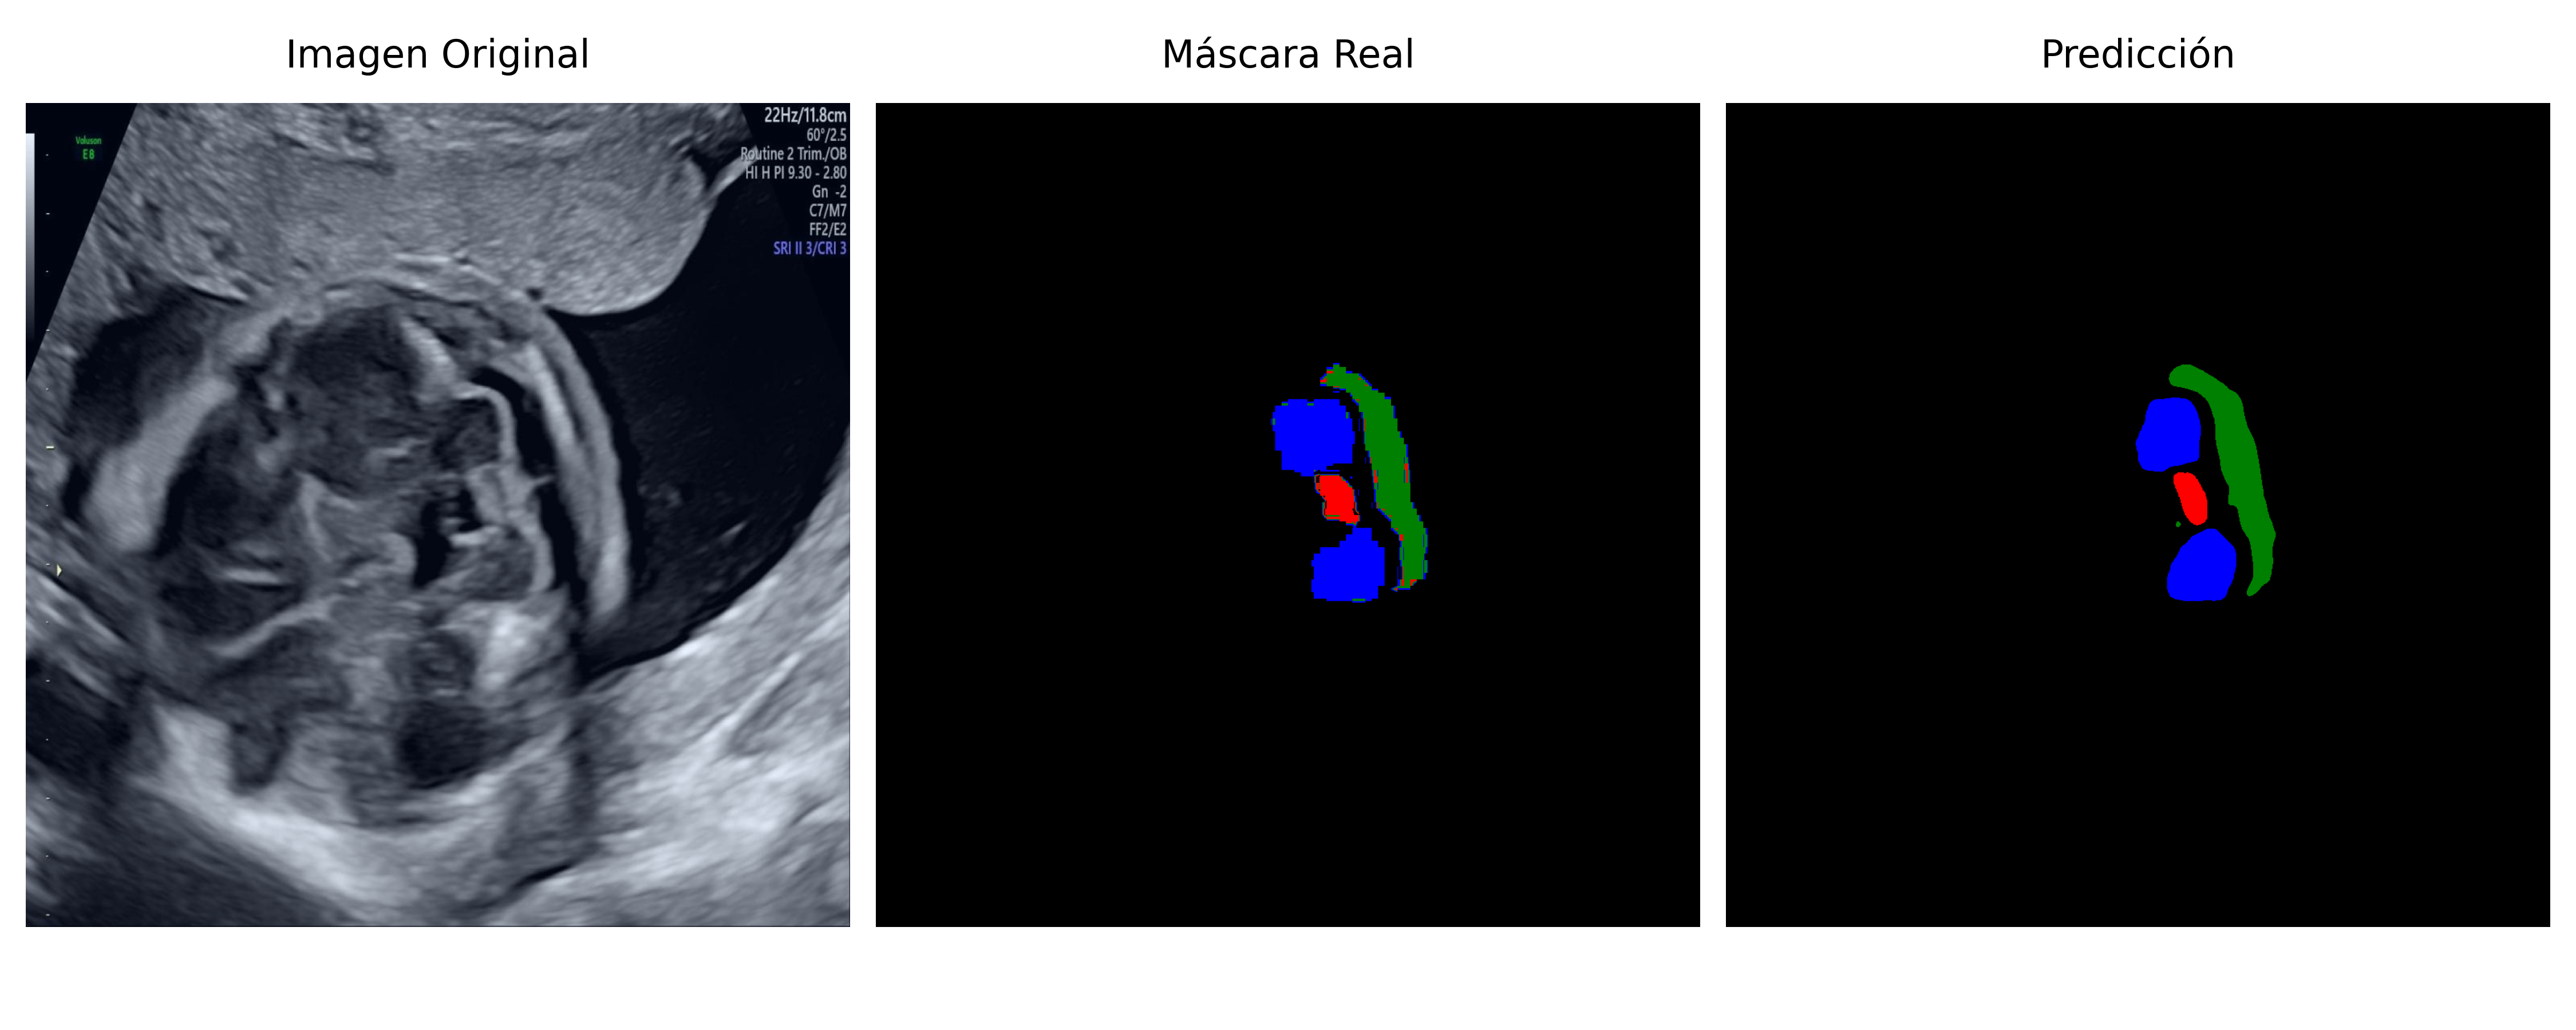
\includegraphics[width=1\textwidth]{img/image4_unet.png}
    \caption{Tercer ejemplo de segmentación con U-Net.}
    \label{fig:comparacion_unet4}
\end{figure}

Como parte del resultado final del proyecto, se desarrolló una interfaz que permite al personal clínico cargar imágenes de ecografía, visualizar las segmentaciones generadas por el modelo, consultar la máscara ground truth cuando está disponible y generar automáticamente informes en formato PDF.

Esta interfaz fue desarrollada inicialmente en \textit{Streamlit} y posteriormente desplegada en la nube mediante \textit{Streamlit Community Cloud}, permitiendo su uso sin necesidad de instalaciones locales. La herramienta está disponible en el siguiente enlace: \url{https://fetalbrainsegmentation.streamlit.app/}.

Las Figuras \ref{fig:subir_imagen}, \ref{fig: visualizar_segmentación}, \ref{fig: generar_informe} muestran capturas de pantalla representativas de la aplicación:

\begin{figure}[h]
    \centering
    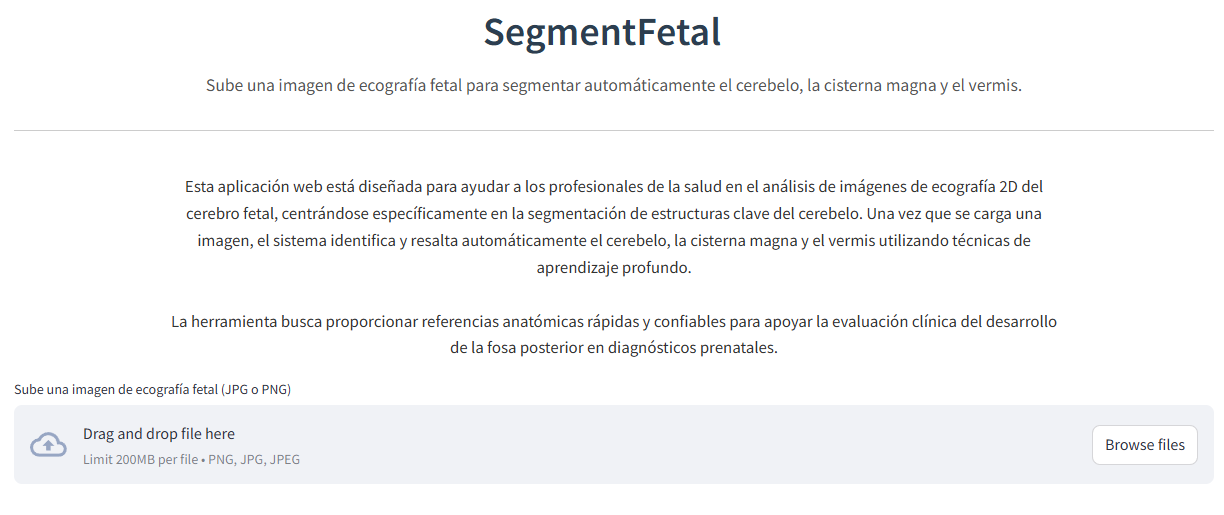
\includegraphics[width=1\textwidth]{img/interfaz_subir_imagen.png}
    \caption{Cargar imagen médica.}
    \label{fig:subir_imagen}
\end{figure}

\begin{figure}[h]
    \centering
    \includegraphics[width=1\textwidth]{img/interfaz_visualización.png}
    \caption{Visualizar segmentación automática.}
    \label{fig: visualizar_segmentación}
\end{figure}

\begin{figure}[h]
    \centering
    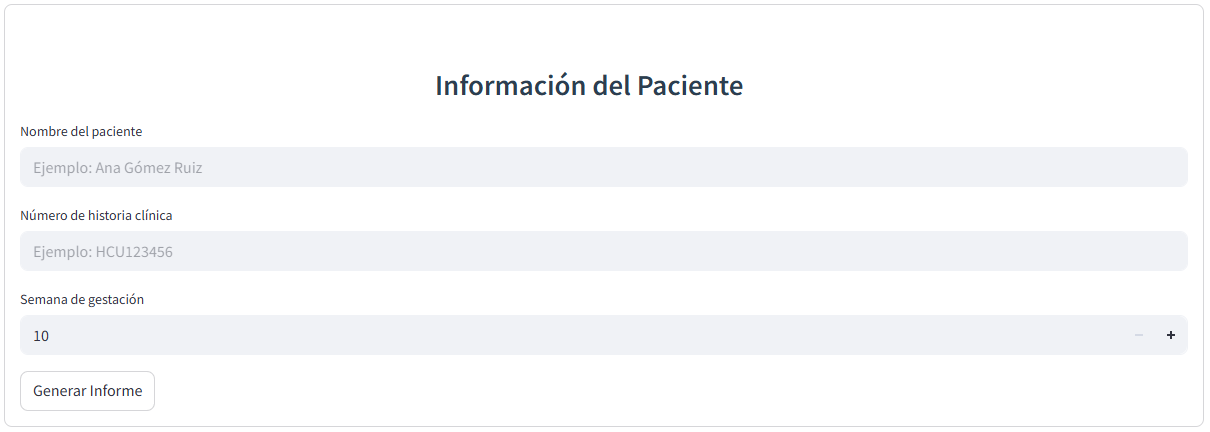
\includegraphics[width=1\textwidth]{img/interfaz_generar_informe.png}
    \caption{Generar informe.}
    \label{fig: generar_informe}
\end{figure}
